
\chapter{基于波动随机照明的透过散射介质超光学记忆效应范围成像}

非侵入式光学成像在从生物成像技术\cite{zhao_non-invasive_2001,artzi_vivo_2011}到光学检测\cite{kozloff_non-invasive_2009}的各个领域都有重要应用。但是,不均匀的样品(例如生物组织)会散射光,从而导致探测器上出现复杂的散斑图案\cite{Goodman1976,Bender}。
随着穿透深度的增加,从散射光中分离出少量的弹道光成为一个很大的挑战\cite{Abramson1978,huang_optical_1991}。多年来,人们提出了许多方法来通过利用或抑制散射光来克服透过散射介质实现非入侵成像的问题。随着空间光调制器的发展,许多方法已经被提出实现控制和操纵散射光的方法\cite{Mosk2012,rotter_light_2017}。目前,已经提出了几种技术来通过使用反馈信号来优化入射光波前来实现聚焦,以重新形成一个焦点,然后利用扫描的方式实现成像\cite{Vellekoop2007,Horstmeyer2015}。这些技术通常需要途径至散射层的两侧获取信号以优化波前,这些条件极大地限制了它们在实际场景中的应用。
为了克服这个问题,已经提出了基于波前整形和各种反馈信号(例如荧光或超声信号)的其他策略\cite{Horstmeyer2015,Katz2019,Popoff2010,Hofer2019},实现波前整形。然而,这些方法要么需要较长的采集时间,要么仅限于小视场 。
另一方面,还提出了几种利用角散斑相关性的技术\cite{bertolotti_non-invasive_2012,katz_non-invasive_2014},即光学记忆效应\cite{Freund1988,Yllmaz2019,Osnabrugge},用于对隐藏在散射介质后面的物体进行成像。这些方法计算散斑图案的自相关,其本质上利用散斑的自相关与隐藏目标的自相关相同,并使用相位检索算法从自相关重建对象图像。虽然这些方法速度很快,但它们的成像范围仍然受到光学记忆效应范围的限制。前面章节中,我们对基于光学记忆效应下的散斑成像进行了原理介绍和实验验证。

线性荧光广泛应用于生物学和生物医学科学\cite{Ruan2020,Lichtman2005,mangeat_super_resolved_2021}。 它能够对细胞、亚细胞或分子成分进行成像,并具有空间分辨率高、对比度高、速度快的优点。近年来,许多技术允许使用荧光通过散射介质进行聚焦和成像。
即便如此,这些方法要么依赖于引导星 \cite{Hhorstmeyer} 的使用,仅限于光学记忆效应范围 \cite{hofer_wide_2018},要么需要表征散射介质 \cite{boniface_non_invasive_2020}。

在本章,我们提出了一种新型的成像方法,该方法使用简单地利用旋转漫射器生成的波动随机散斑照明,允许透过散射介质在一定深度上远远超出光学记忆效应范围的进行非侵入性成像。当随机照明散斑产生后,每个荧光发射器都会在探测器上产生独特的散斑图案,我们称其为“散斑指纹”。相机所捕获的每张图像都是来自不同荧光发射器的所产生的散斑指纹的非相干总和。当随机照明随着旋转器改变时,探测器上所接收的散斑的各个散斑指纹的权重随之改变。为了检索每个单独的指纹,我们在随机改变光照的同时捕获一组图像,并使用非负矩阵分解 (Non-negative Matrix Factorization,NMF) 算法对采集的数据进行去混叠。随后,通过探索指纹之间的相关性,使用指纹重建最终图像。为了验证该技术的有效性,我们通过实验证明了我们在荧光珠和连续荧光物体上的非侵入性成像方法。

\section{基于波动随机照明的透过散射介质超光学记忆效应范围成像基本原理}

\begin{figure}[htp]
	\centering
	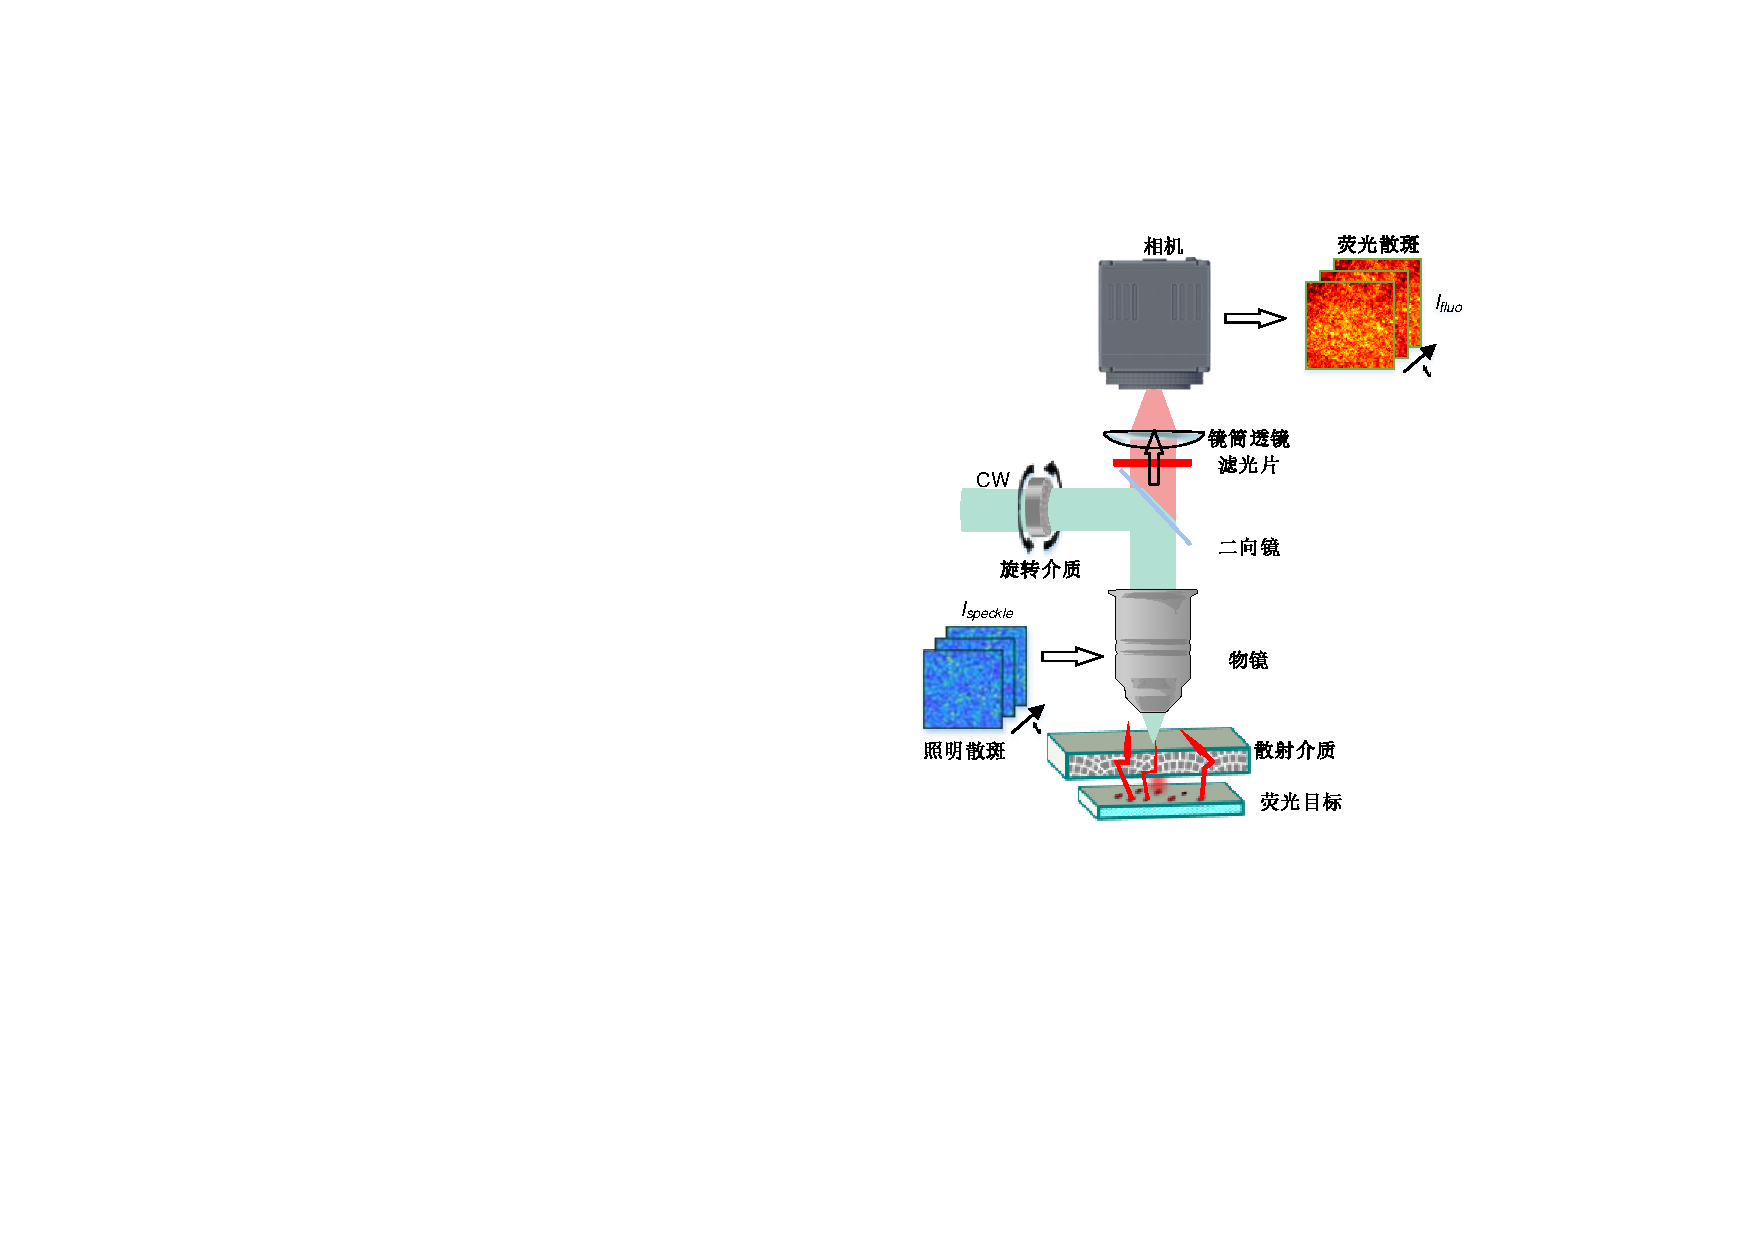
\includegraphics[scale=0.75]{C5.fig1}
	\caption{非入侵成像系统示意图}
	\label{fig:5.1}
\end{figure}

非入侵成像系统如图\ref{fig:5.1}所示。当激光通过旋转漫反射器时,入射激光被添加了随机相位实现了入射激光的随机调制,进而调制光透过散射介质产生了未知的随机散斑,未知的散斑照明目标。利用随机散斑照明目标后,目标产生自身的激发光,激发光传播并通过散射介质,产生散斑最终被相机所接收,此时相机所获得的散斑为不同散斑指纹的非相干总和。尽管捕获的图像对比度低、随机且看似无信息,但它们包含来自对象独立发射器的所有散斑指纹,且其各自的权重随着随机照明的改变具有时间的多样性。此外,光学记忆效应范围内的独立发射器将在相机上产生相关但平移的散斑指纹 \cite{Freund1988},而光学记忆效应范围外的发射器将产生完全不相关的散斑指纹。对于给定的散斑照明,捕获的图像 $I_{\textsl{fluo}}$ 可以表示为具有不同权重的散斑指纹的线性叠加。因此,相机图像$I_{\textsl{fluo}}$由下式给出:

\begin{equation}
\begin{aligned}
I_{fluo}(r,t) = \sum^{P}_{k=1} w_{k}(r) h_{k}(t),
\label{eq:5.1}
\end{aligned}
\end{equation}
其中, $I_{fluo}(r,t)$为对应于第$t$次照明时相机所接收到低对比度散斑,$r$为空间坐标,$w_{k}(r)$为第$k$个独立发射器所对应的散斑指纹,$h_{k}(t)$为第$t$次照明时第$k$个独立发射器所接收到的激光光的强度,$P$为系统中独立发射器的数量。

当拥有足够多的随机散斑照明时,就可以采集到足够的低对比度散斑图案,通过NNF对散斑集进行去混叠,获得各自发射器的散斑指纹。然后利用,指纹重建算法实现最终图像的重建。整体流程下所示;
\begin{algorithm2e}[h!]
\DontPrintSemicolon
\SetAlgoLined
\KwInput{系列散斑图案, $I_{fluo}(r,t)$.}
\KwOutput{隐藏目标的图像, $O^{Global}$.}
从系列数据集$I_{fluo}(r,t)$估计系统的秩($\rho$).\;

通过去混叠算法恢复散斑指纹($w_{i}$).\;

\For{$k=1,...,\rho$}{
在指纹$w_{k}$和其余所有的指纹($w_{i\neq k}$)之间进行成对去卷积运算.\;

获取位于与散斑指纹$w_{k}$所对应的独立发射器同一光学记忆效应范围内的独立发射器之间的相对位置.\;

获得局部重建结果($O_{k}$).\;
}

将不同区域的局部重建结果($O_{k}$)合成全局重建结果($O^{Global}$).\;

\caption{非入侵图像重建流程}
\label{alg:a1}
\end{algorithm2e}

\subsection{散斑指纹去混叠}


\begin{figure}[htp]
	\centering
	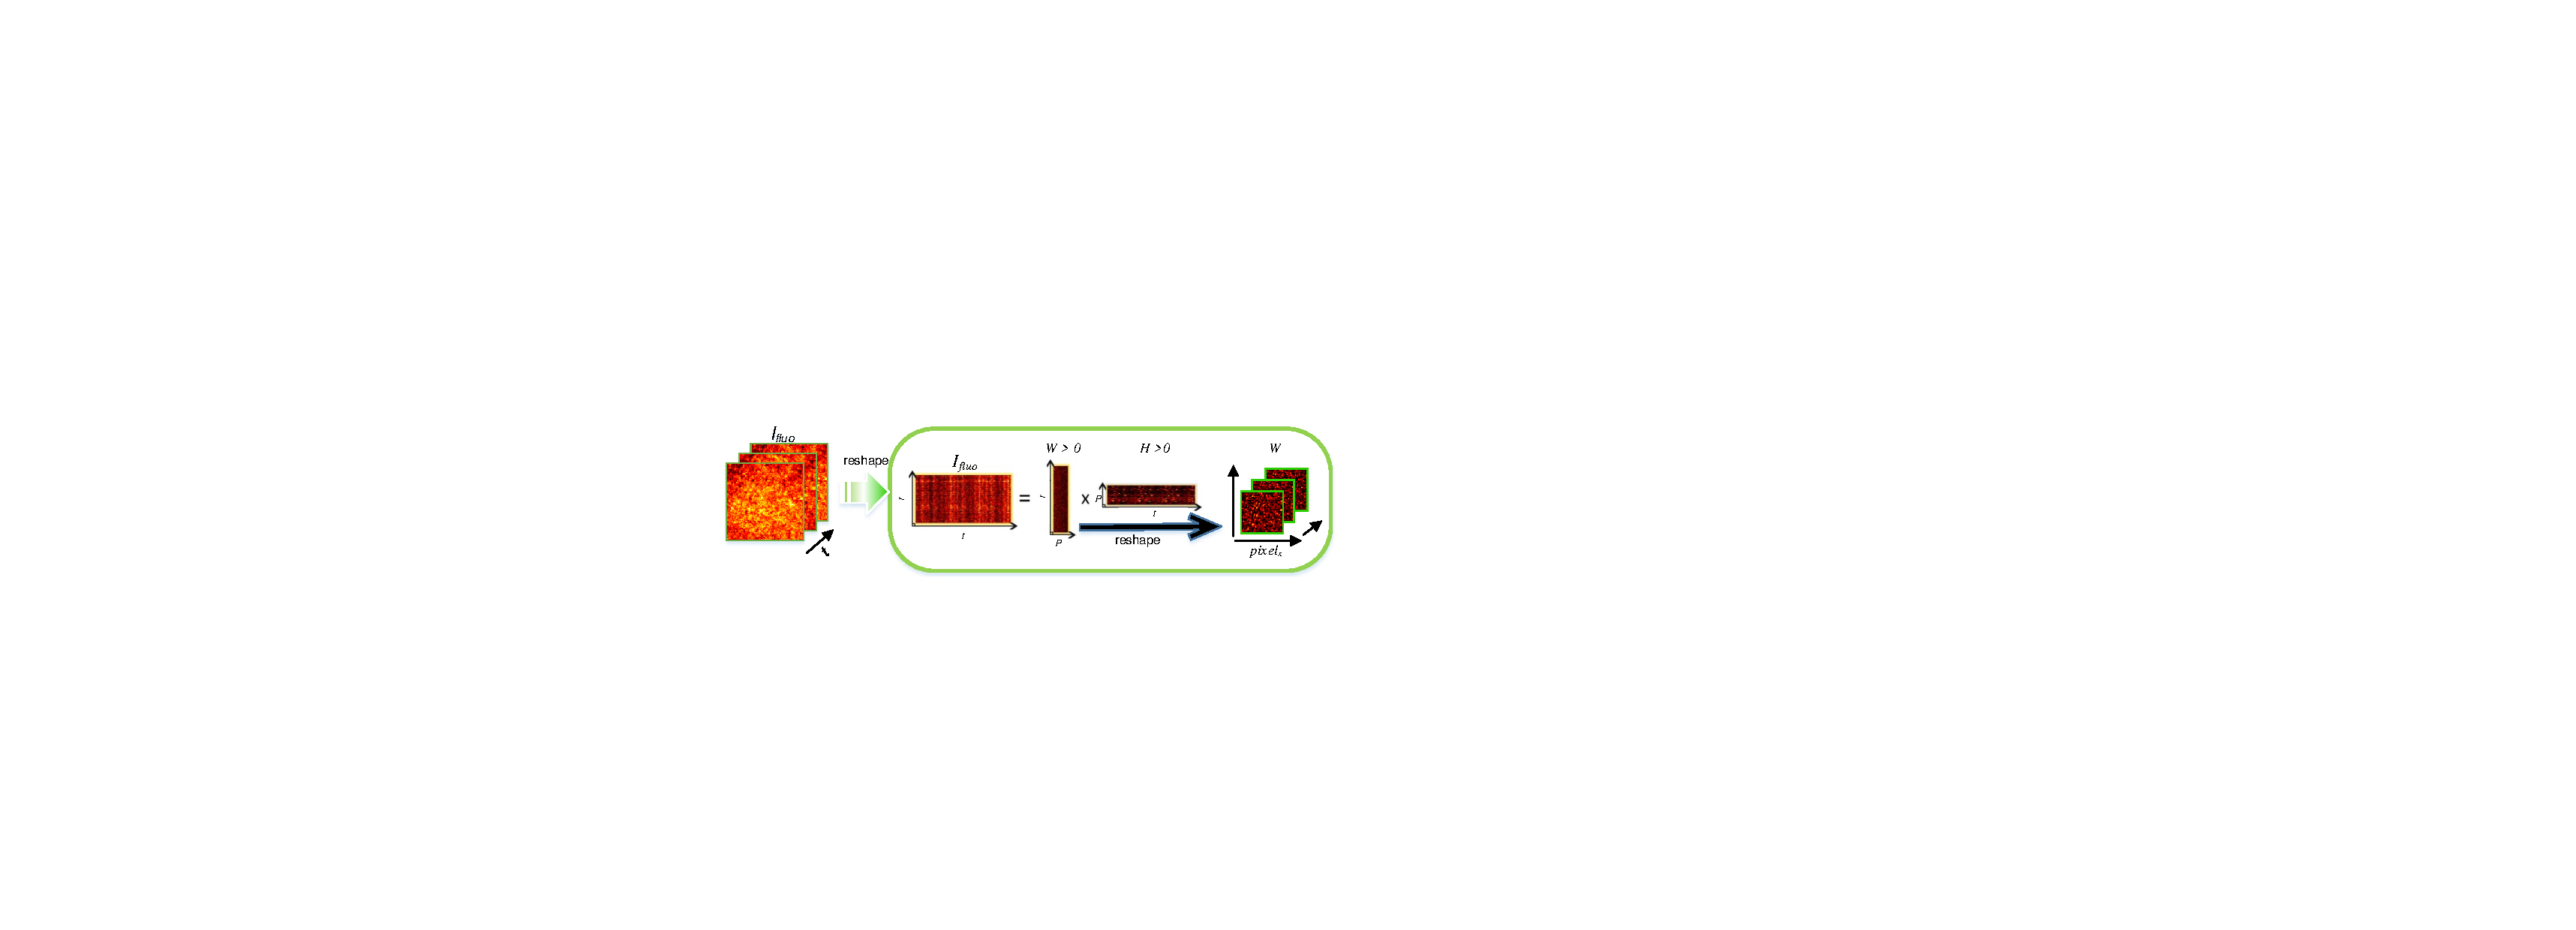
\includegraphics[scale=1.0]{C5.fig2}
	\caption{散斑指纹去混叠过程}
	\label{fig:5.2}
\end{figure}

\begin{figure}[htp]
	\centering
	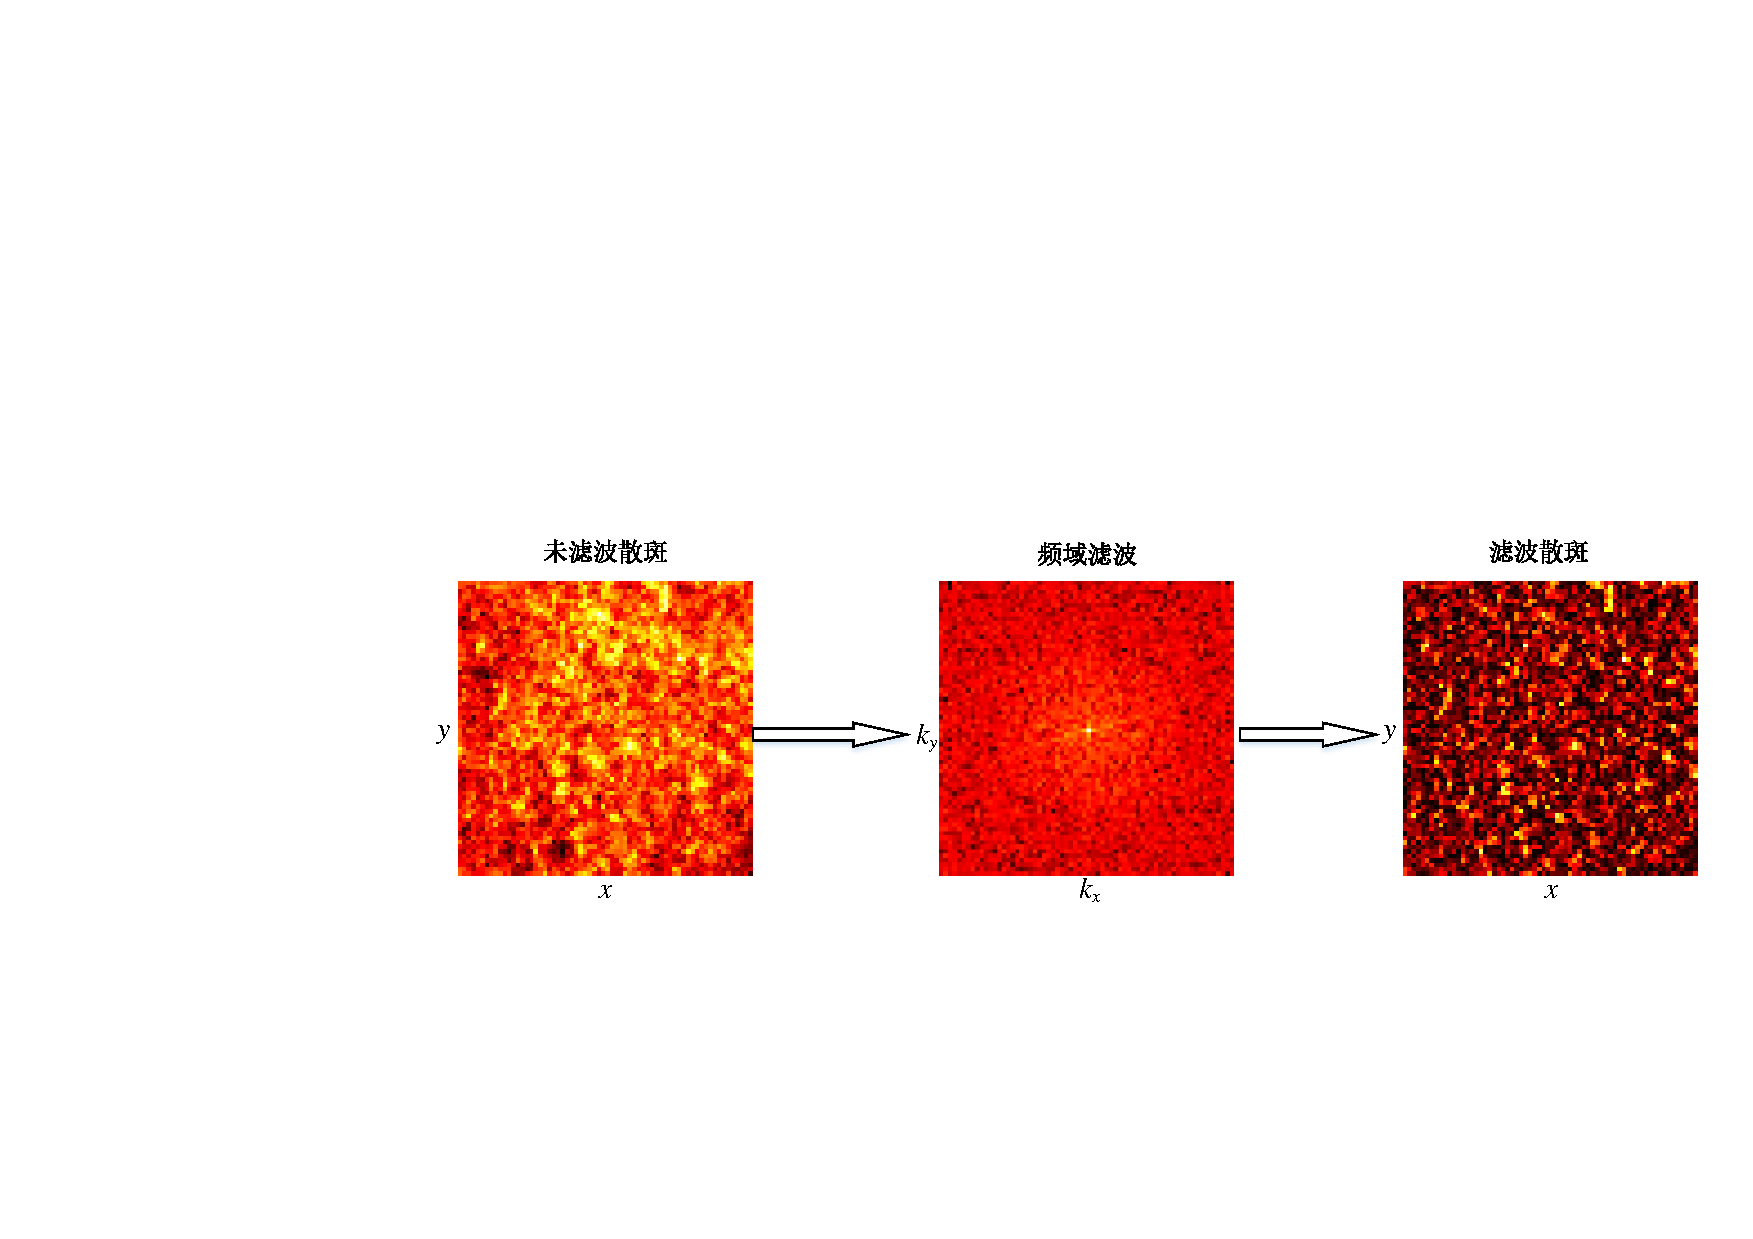
\includegraphics[scale=0.5]{C5.fig3}
	\caption{散斑滤波}
	\label{fig:5.3}
\end{figure}
